\documentclass{article}
\usepackage{tikz}
\usetikzlibrary{positioning}

\tikzset{
    block/.style={
        draw,
        rounded corners,
        minimum width=2.6cm,
        minimum height=1cm,
        align=center,
        fill=blue!10
    },
    neuron/.style={
        circle,
        draw,
        minimum size=8mm
    },
    line/.style={
        ->,
        thick,
        red
    }
}

\begin{document}

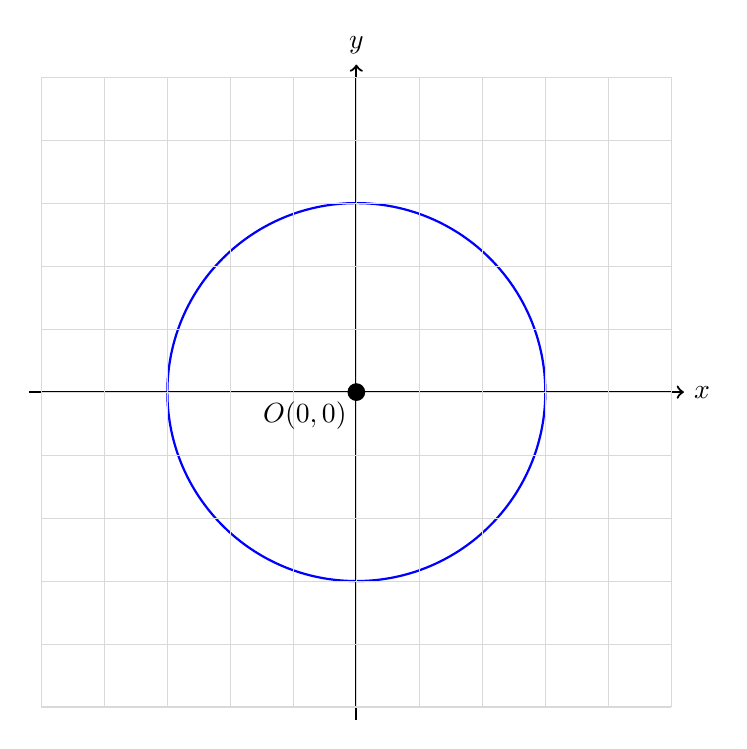
\begin{tikzpicture}[scale=0.8]

    \draw[blue, thick] (0,0) circle (3);

    \draw[->, thick] (-5.2,0) -- (5.2,0) node[right] {$x$};
    \draw[->, thick] (0,-5.2) -- (0,5.2) node[above] {$y$};

    \draw[step=1cm, gray!30, thin] (-5,-5) grid (5,5);

    \fill (0,0) circle (4pt);
    \node[below left] at (0,0) {$O(0,0)$};

\end{tikzpicture}

\newpage

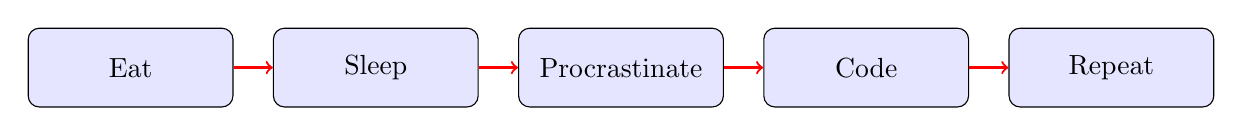
\begin{tikzpicture}[node distance=0.5cm]

    \node[block] (eat) {Eat};
    \node[block, right=of eat] (sleep) {Sleep};
    \node[block, right=of sleep] (procrastinate) {Procrastinate};
    \node[block, right=of procrastinate] (code) {Code};
    \node[block, right=of code] (repeat) {Repeat};

    \draw[line] (eat) -- (sleep);
    \draw[line] (sleep) -- (procrastinate);
    \draw[line] (procrastinate) -- (code);
    \draw[line] (code) -- (repeat);

\end{tikzpicture}

\newpage

\begin{tikzpicture}

    \foreach \x in {0,...,4}{
        \foreach \y in {0,...,4}{
            \draw (2*\x,2*\y) rectangle ++(1,1);
        }
    }

\end{tikzpicture}

\newpage

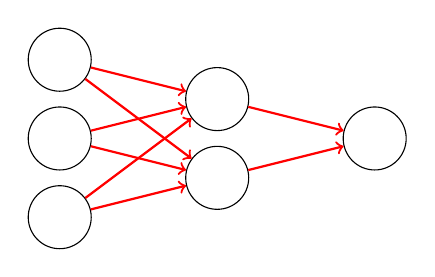
\begin{tikzpicture}

\foreach \y in {0,1,2}
    \node[neuron] (I\y) at (0,{2-\y}) {};

\foreach \y in {0,1}
    \node[neuron] (H\y) at (2,{1.5-\y}) {};

\node[neuron] (O0) at (4,1) {};

\foreach \i in {0,1,2}
    \foreach \h in {0,1}
        \draw[line] (I\i) -- (H\h);

\foreach \h in {0,1}
    \draw[line] (H\h) -- (O0);

\end{tikzpicture}

\end{document}
